%% arara directives
% arara: xelatex
% arara: bibtex
% arara: xelatex
% arara: xelatex

%\documentclass{article} % One-column default
\documentclass[twocolumn, switch]{article} % Method A for two-column formatting

\usepackage{preprint}

%% Math packages
\usepackage{amsmath, amsthm, amssymb, amsfonts}

%% Bibliography options
\usepackage[numbers,square]{natbib}
\bibliographystyle{unsrtnat}
%\usepackage{natbib}
%\bibliographystyle{Geology}

%% General packages
\usepackage[utf8]{inputenc}	% allow utf-8 input
\usepackage[T1]{fontenc}	% use 8-bit T1 fonts
\usepackage{xcolor}		% colors for hyperlinks
\usepackage[colorlinks = true,
            linkcolor = purple,
            urlcolor  = blue,
            citecolor = cyan,
            anchorcolor = black]{hyperref}	% Color links to references, figures, etc.
\usepackage{booktabs} 		% professional-quality tables
\usepackage{nicefrac}		% compact symbols for 1/2, etc.
\usepackage{microtype}		% microtypography
\usepackage{lineno}		% Line numbers
\usepackage{float}			% Allows for figures within multicol
%\usepackage{multicol}		% Multiple columns (Method B)

\usepackage{graphicx}		%  Images
\graphicspath{.}

 %% Special figure caption options
\usepackage{newfloat}
\DeclareFloatingEnvironment[name={Supplementary Figure}]{suppfigure}
\usepackage{sidecap}
\sidecaptionvpos{figure}{c}

% Section title spacing  options
\usepackage{titlesec}
\titlespacing\section{0pt}{12pt plus 3pt minus 3pt}{1pt plus 1pt minus 1pt}
\titlespacing\subsection{0pt}{10pt plus 3pt minus 3pt}{1pt plus 1pt minus 1pt}
\titlespacing\subsubsection{0pt}{8pt plus 3pt minus 3pt}{1pt plus 1pt minus 1pt}

% ORCiD insertion
\usepackage{tikz,xcolor,hyperref}

\definecolor{lime}{HTML}{A6CE39}
\DeclareRobustCommand{\orcidicon}{
	
\begin{tikzpicture}
	\draw[lime, fill=lime] (0,0) 
	circle [radius=0.16] 
	node[white] {{\fontfamily{qag}\selectfont \tiny ID}};
	\draw[white, fill=white] (-0.0625,0.095) 
	circle [radius=0.007];
	\end{tikzpicture}
	\hspace{-2mm}
}
\foreach \x in {A, ..., Z}{\expandafter\xdef\csname orcid\x\endcsname{\noexpand\href{https://orcid.org/\csname orcidauthor\x\endcsname}
			{\noexpand\orcidicon}}
}
% Define the ORCID iD command for each author separately. Here done for two authors.
\newcommand{\orcidauthorA}{0000-0000-0000-0001}
\newcommand{\orcidauthorB}{0000-0000-0000-0002}
\newcommand{\orcidauthorC}{0000-0000-0000-0003}
\newcommand{\orcidauthorD}{0000-0000-0000-0004}

%%%%%%%%%%%%%%%%   Title   %%%%%%%%%%%%%%%%
\title{AUTOBRICK: A system for end-to-end automation of building point labels to Brick turtle files}

% Add watermark with submission status
\usepackage{xwatermark}
% Left watermark
\newwatermark[firstpage,color=gray!60,angle=90,scale=0.32, xpos=-4.05in,ypos=0]{\href{https://doi.org/}{\color{gray}{Publication doi}}}
% Right watermark
\newwatermark[firstpage,color=gray!60,angle=90,scale=0.32, xpos=3.9in,ypos=0]{\href{https://doi.org/}{\color{gray}{Preprint doi}}}
% Bottom watermark
\newwatermark[firstpage,color=gray!90,angle=0,scale=0.28,
xpos=0in,ypos=-5in]{*correspondence: \texttt{dbdesai@ucsd.edu}}

%%%%%%%%%%%%%%%  Author list  %%%%%%%%%%%%%%%
\usepackage{authblk}
\renewcommand*{\Authfont}{\bfseries}
\author[1\thanks{dbdesai@ucsd.edu}]{Devanshu Desai\orcidA{}}
\author[2\thanks{agemawat@ucsd.edu}]{Advitya Gemawat\orcidB{}}

\affil[1]{Halicoglu Data Science Institute, University of California at San Diego}
\affil[2]{Halicoglu Data Science Institute, University of California at San Diego}

% Option 2 for author list
%\author{
%  David S.~Hippocampus\thanks{Use footnote for providing further
%    information about author (webpage, alternative
%    address)---\emph{not} for acknowledging funding agencies.} \\
%  Department of Computer Science\\
%  Cranberry-Lemon University\\
%  Pittsburgh, PA 15213 \\
%  \texttt{hippo@cs.cranberry-lemon.edu} \\
%  %% examples of more authors
%   \And
% Elias D.~Striatum \\
%  Department of Electrical Engineering\\
%  Mount-Sheikh University\\
%  Santa Narimana, Levand \\
%  \texttt{stariate@ee.mount-sheikh.edu} \\
%  \AND
%  Coauthor \\
%  Affiliation \\
%  Address \\
%  \texttt{email} \\
%  % etc.
%}

%%%%%%%%%%%%%%    Front matter    %%%%%%%%%%%%%%
\begin{document}

\twocolumn[ % Method A for two-column formatting
  \begin{@twocolumnfalse} % Method A for two-column formatting
  
\maketitle

\begin{abstract}
    BRICK is a schema for representing various building equipment,
    including but not limited to, HVAC air handling units and carbon dioxide
    sensors in different rooms. While the schema is a clear step up over the
    current state-of-the-art, its potential is severely hindered because
    it is not backwards compatible. This means that converting \texttt{CSV}
    files storing building data to a BRICK-compatible data format is a
    cumbersome and imperfect process as different systems use different
    conventions to denote the same systems. This conversion usually required
    human involvement until now. AUTOBRICK is a software tool that automates
    this conversion with minimal human intervention and provides an order
    of magnitude greater speed up (90x) over the current state of the art.
\end{abstract}
%\keywords{First keyword \and Second keyword \and More} % (optional)
\vspace{0.35cm}

  \end{@twocolumnfalse} % Method A for two-column formatting
] % Method A for two-column formatting

%\begin{multicols}{2} % Method B for two-column formatting (doesn't play well with line numbers), comment out if using method A


%%%%%%%%%%%%%%%  Main text   %%%%%%%%%%%%%%%
% \linenumbers

\section{Introduction}
Today, several commercial buildings have sought to leverage the power of
cyber-physical systems for optimal energy consumption, planned facility
maintenance, machine learning (ML) applications, etc., to augment user
experience. However, their data collection / ETL methodologies don’t conform to
a uniform schema to enable buildings to ‘interact’ with each other or
streamline the process of analytics and ML at scale. The US building industry
suffers a loss of \$1.5B / year due to the lack of interoperable warehousing
between different buildings \cite{balaji_2016}. Brick offers a comprehensive
schema to represent arbitrary buildings metadata, build programmatic platforms
for commercial buildings, improve interoperability between different buildings,
and pave the way for well-defined ways of analyses related to planned
maintenance and machine learning, etc. \cite{balaji_2016}. 

Converting arbitrary metadata schema to Brick (i.e., \emph{'Brickification'}) is a
slow process bogged down by manual interventions into partially-automated
processes and grunt work. This process involves custom data transformations,
object-relationship definitions, and manually plugging intermediate results
into various heterogeneous frameworks to get a \texttt{Turtle} file parseable by Brick.
A \texttt{Turtle} file is a data format that expresses data in a RDF model which can be used to store graph-like info for
relationships between different entities, in this case, building sub-systems and
sensors. Different kinds of building point label (metadata string) formats that sabotage the notion of a ‘one-size fits all’ solution further intensify these challenges.  Additionally, this is also motivated by real-life use cases such as the COVID-19 global pandemic, where the public safety regulations in indoor environments (classrooms, offices, etc.) remain a massively unsolved research question and challenge at scale.


\section{Background}

The traditional Brickification workflow involves:
\begin{enumerate}
    \item an open-source Excel-like tool called ‘\emph{OpenRefine},’ where users need
        to perform manual data transformations
        \cite{gtfierro225_2020},
    \item a ‘\emph{Reconciliation API},’ to infer the class of specific objects in
        terms of Brick’s vocabulary \cite{brickschema},
    \item Entity-relationship definitions in a \texttt{.txt} file, to utilize in the
        turtle file \cite{gtfierro}, and
    \item a tool called ‘\emph{Brick Builder}’ to convert the processed data into its
        turtle file \cite{brick_ttl_viewer}.
\end{enumerate}
As symbolized in Figure \ref{fig:fig1}, the data transformations and most of the API injections and integrations need to be manually done by the user. The BrickBuilder tool is the only component to automate the last part of this workflow. We recognize the research and practical utility of the frameworks already created for use in the old Brickification workload. We don’t seek to reinvent the wheel here but address automation, acceleration, and scalability improvements on top of these existing systems.

\begin{figure}[H]
  \centering
  \fbox{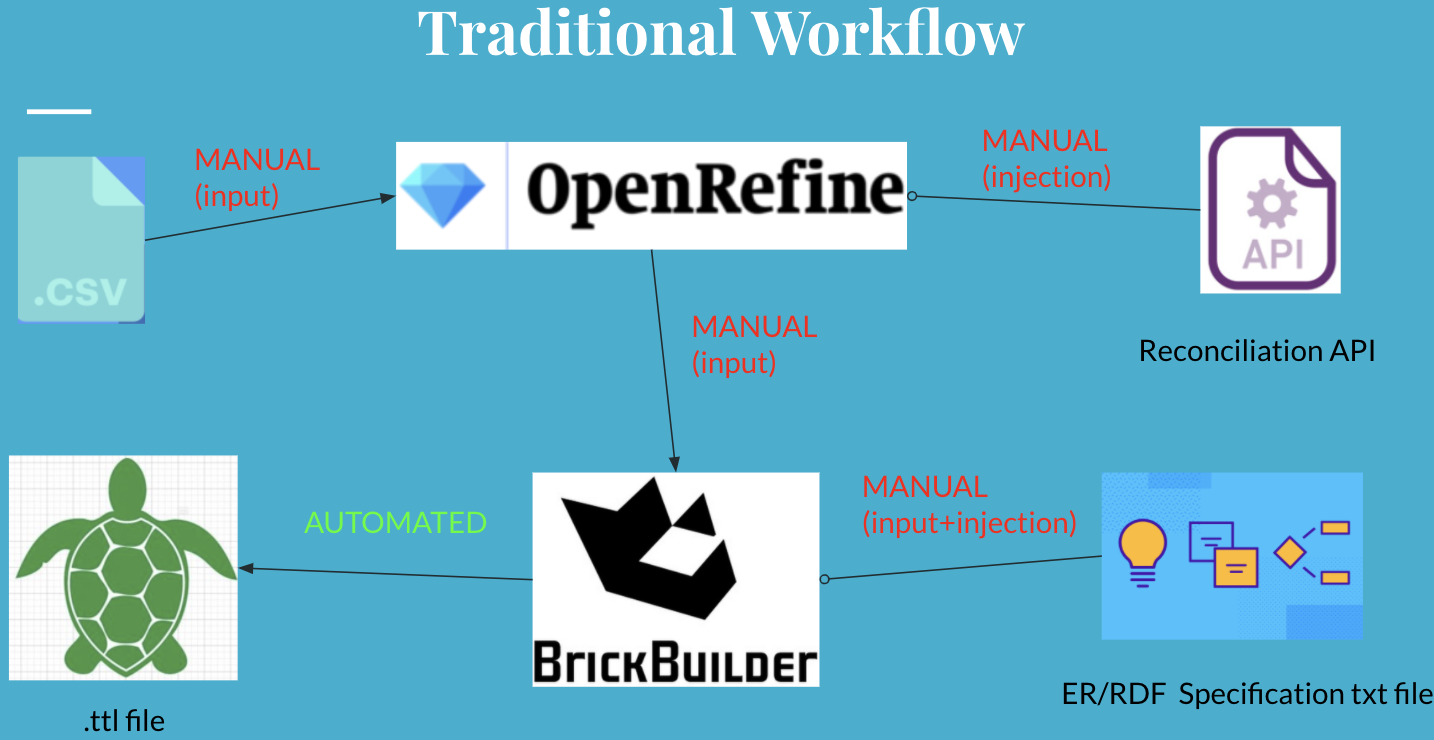
\includegraphics[scale=0.17]{traditional_workflow.png}}
  \caption{ Traditional pre-existing Brickification workflow as per the
  tutorial in \cite{gtfierro225_2020} }
  \label{fig:fig1}
\end{figure}

\section{Our Framework}

\begin{figure}[H]
  \centering
  \fbox{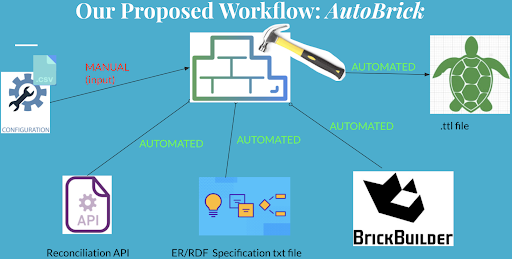
\includegraphics[scale=0.45]{autobrick_workflow.png}}
  \caption{The proposed workflow through AUTOBRICK}
  \label{fig:fig2}
\end{figure}

‘AUTOBRICK’ is an end-to-end system for automating and accelerating the
conversion of point labels into turtle files with Brick terminology, which can
be visualized, queried, and utilized by the Brick programming platform. As
displayed in Figure \ref{fig:fig2}, the tool takes a configuration file where users can declaratively specify all details about their data and workload (related to data location, point label format details, and additional parsing details). AUTOBRICK automates all needed data transformations to pre-process the point labels and extract relevant information of various units/sensors and categories related to specific building objects. AUTOBRICK utilizes pre-written / pre-loaded standard ER/RDF specifications and existing APIs to inject and stitch them on the pre-processed data as per the original sequence of steps followed for Brickification. We recognize the research and practical utility of the frameworks already created for use in the old Brickification workload and address automation, acceleration, and scalability improvements on top of the existing implementations. 

	AUTOBRICK allows for flexibility in using arbitrary \texttt{CSV} files and
    chosen/specified point label formats. With the project, we give the power
    in the user’s hands for them to decide the appropriate dataset
    parsing/preprocessing strategies, rather than making unverified assumptions
    about point label structures or utilizing unreliable custom static analysis
    or auto-generation techniques. AUTOBRICK has already \emph{"brickified}" 41 point
    label datasets of various buildings in UCSD’s Engineering Department,
    reducing the need for human intervention to a matter of minutes. Initial
    experiments and demos have already showcased \emph{Autobrickify} reducing
    \emph{~10-15 mins} of manual grunt work as part of \emph{"brickifying}" one dataset (as part of
    the tutorial in \cite{gtfierro225_2020}) to a matter of \emph{<10 seconds}, 
    achieving orders-of-magnitude \textbf{(over 90x)} speed-ups and scalability!

\section{Methods}
We use a combination of \texttt{Python} and shell scripts to execute the workload in terms of the core logic to parse the point labels and loading and injecting pre-existing APIs at different stages of the process.  
To automate data transformations, we use the pandas module to load the data in
memory and leverage the supplied configurations to perform data manipulations
with in-built functions provided by the module to identify objects/pieces of
equipment such as \emph{AHU}s, \emph{Zone}s, \emph{VAV}s, and their corresponding class types. 

	Utilizing shell, we write some custom scripts to clone the APIs, load them in the execution environment, and call them according to their instructions to supply the pre-processed data to their API function calls automatically.  
    Because modules such as \texttt{Pandas} are pre-installed in a standard
    \texttt{Python} environment, the tool doesn’t have any unique dependencies. It just needs to rely on the brick-builder API’s dependencies (i.e., two modules, brickschema and rdflib). The lack of dependencies further makes the tool lightweight for smooth usage. The requirements are directly taken (and hence can even be updated) from the loaded APIs themselves, making it seamless to piggyback on top of the APIs made for Brickification.

\begin{figure}[H]
  \centering
  \fbox{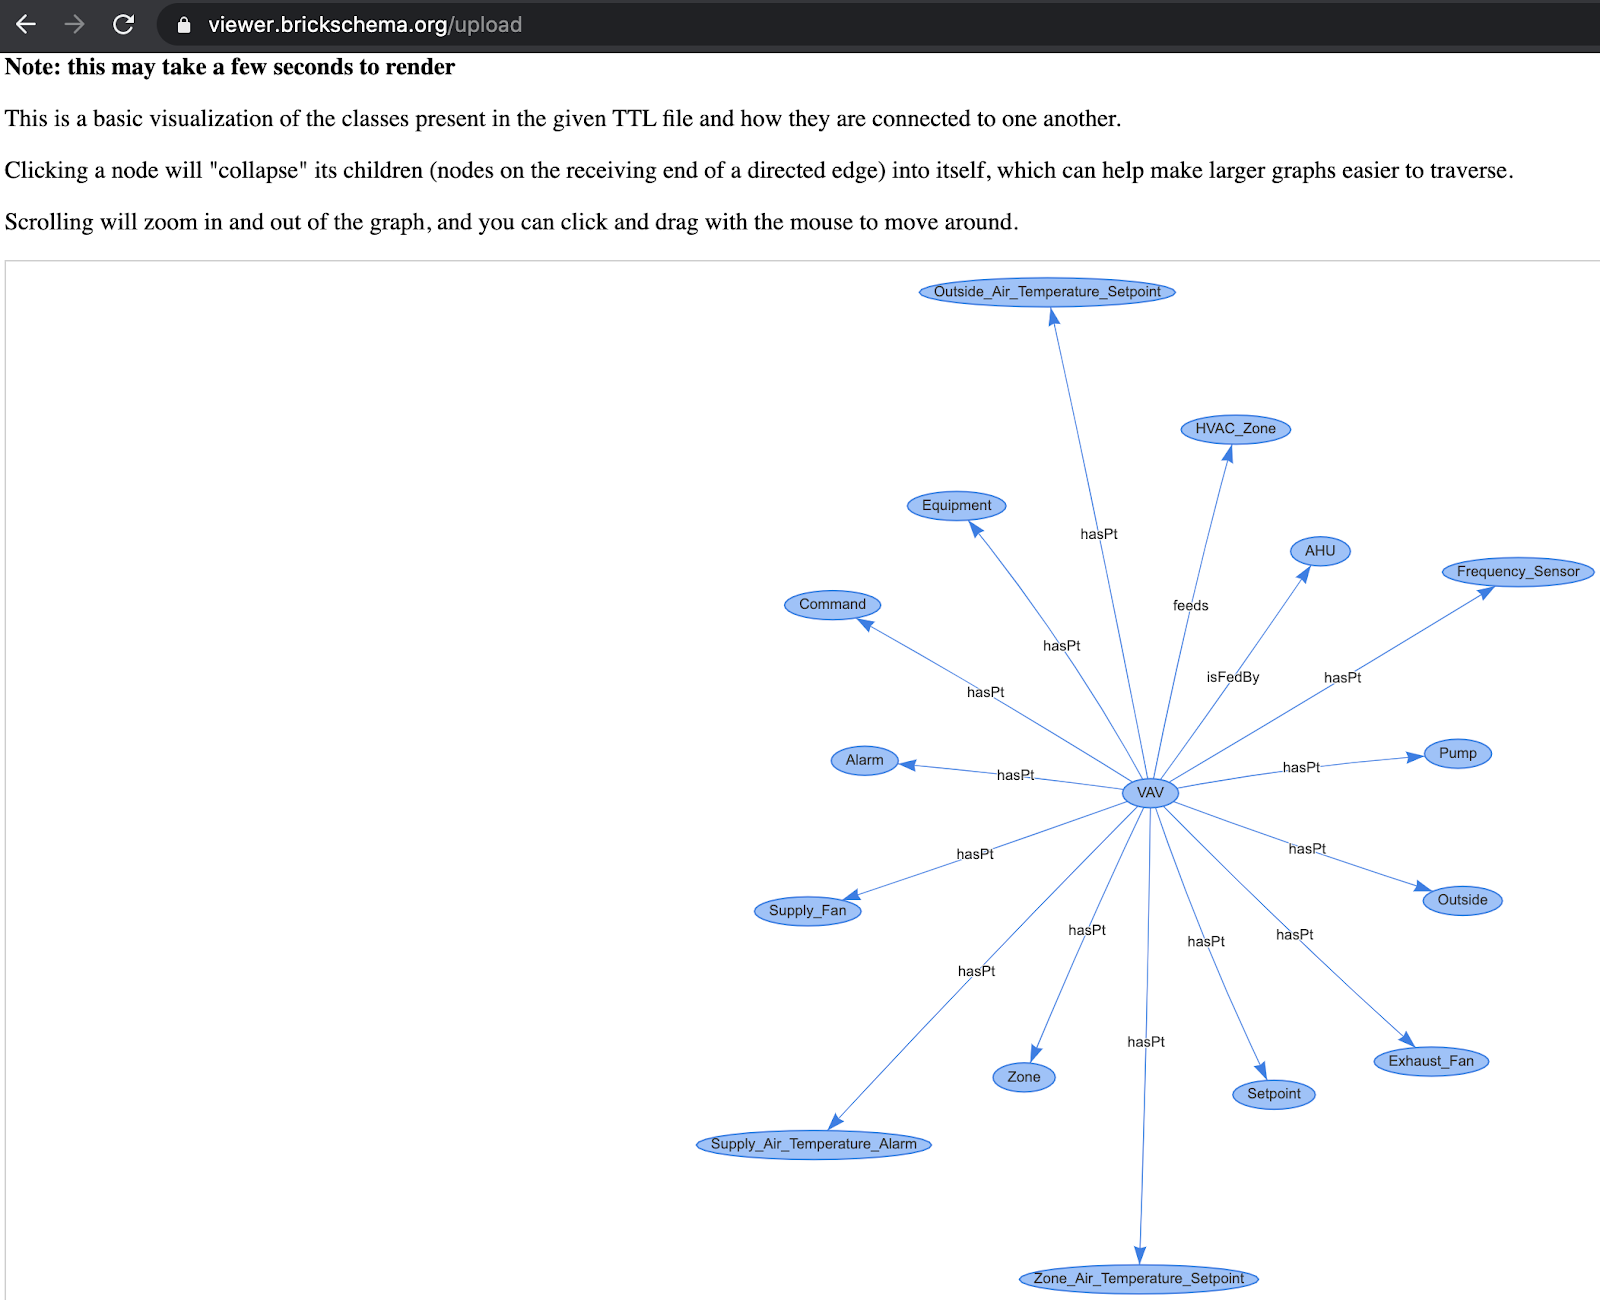
\includegraphics[scale=0.15]{brick_viewer.png}}
  \caption{We can also use the Brick Viewer tool
  \cite{brick_ttl_viewer} to eyeball the relationship graph of the building sub-systems.}
  \label{fig:fig3}
\end{figure}


Our validation process involves both automated and manual aspects. Since we don't have any target files to compare our outputs with, we use domain experts working under our mentor. Domain experts carefully go through the generated turtle files and verify if the outputs match their expectations. The automated component involves running some automated test queries on the generated files to ensure that the graphical model can be parsed error-free, and we’ve showcased some of such queries in one of our demos as well.

\section{Work Extensions}
One of the biggest challenges faced in the Brickification workflow is the
predictions of Brick Classes by the \emph{Reconciliation API}, which have only been
around 30\% accurate \cite{gtfierro225_2020}. The \emph{Reconciliation API} uses an extensive key-value pair dictionary to extract and attach relevant ontology for a sensor abbreviation in a point label, but the API isn’t comprehensive. Ultimately, the turtle files need to be precisely correct for effective ETL and Analytics utilization. To mitigate this, we also formulated scripts to extract additional key-value pairs from Johnson Controls’ documentation to update the API and get more accurate predictions. However, this process of incorporating all key-value pairs may never be fully comprehensive and is subject to future updates. On the bright side, AUTOBRICK directly uses the latest version of the API, automatically reflecting better results as the API improves. 

	The second part of augmenting the tool’s robustness relates to dealing with point label values with an unequal number of splits with the specified delimiters. In our current implementation, we assume the point labels split into a uniform number of elements. For point labels that split into fewer values, we consider these point-labels invalid (as we did encounter spurious point label values during our testing). Filtering out these point-labels renders the remaining values invalid. During the preprocessing stage, we drop rows with any null values. In other words, we treat point labels with the maximum number of splits possible in the dataset as the only legitimate kind of point label value for that dataset. Dealing with diverse but correct formats of point labels in a single dataset is an open research question needing collaboration with domain experts and is left to future work.

Finally, we also implemented a virtual reality front end to interact and
query with the automatically generated turtle files. The environment is set up
as a scene on a platform called ARENA \cite{conix-center}. We set up a server that listens for
events and user interactions with the 3D objects in ARENA and translates those
interactions into queries performed on the BRICK-compatible building
information. This environment allows us to map physical spaces into equivalent virtual ones.

\section{Results and Conclusion}
AUTOBRICK automates and accelerates a painfully manual process, thereby
empowering building management and vendors to truly realize the power of
data-driven applications and advanced analytics to augment user experience in
commercial buildings. AUTOBRICK also gives rise to the potential of
representing building sub-systems as virtual spaces to reduce the need for
engineers to physically climb into the building's HVAC system equipment and virtually observe and ‘interact’ with sensor setpoints. To truly reap the benefits of AUTOBRICK, the workflow and use case coverage need to be continually examined by domain experts and industry practitioners to ensure the tool meets their needs at all times. This paper aims to set the foundation for tangibly realizing ‘smart’ buildings and adopt technological advancements moving forward.

% \paragraph{Paragraph}
% \lipsum[7]

% \section{Examples of citations, figures, tables, references}
% \label{sec:others}
% \lipsum[8] \cite{kour2014real,kour2014fast} and see \cite{hadash2018estimate}.

% The documentation for \verb+natbib+ may be found at
% \begin{center}
%   \url{http://mirrors.ctan.org/macros/latex/contrib/natbib/natnotes.pdf}
% \end{center}
% Of note is the command \verb+\citet+, which produces citations
% appropriate for use in inline text.  For example,
% \begin{verbatim}
%    \citet{hasselmo} investigated\dots
% \end{verbatim}
% produces
% \begin{quote}
%   Hasselmo, et al.\ (1995) investigated\dots
% \end{quote}

% \begin{center}
%   \url{https://www.ctan.org/pkg/booktabs}
% \end{center}


% \subsection{Figures}
% \lipsum[10] 
% See Figure \ref{fig:fig1}. Here is how you add footnotes. %\footnote{Sample of the first footnote.}
% \lipsum[11] 

% \begin{figure}[H]
%   \centering
%   \fbox{\rule[-.5cm]{4cm}{4cm} \rule[-.5cm]{4cm}{0cm}}
%   \caption{Sample figure caption.}
%   \label{fig:fig1}
% \end{figure}

% \subsection{Tables}
% \lipsum[12]
% See awesome Table \ref{tab:table}.

% \begin{table}[H]
%  \caption{Sample table title}
%   \centering
%   \begin{tabular}{lll}
%     \toprule
%     \multicolumn{2}{c}{Part}                   \\
%     \cmidrule(r){1-2}
%     Name     & Description     & Size ($\mu$m) \\
%     \midrule
%     Dendrite & Input terminal  & $\sim$100     \\
%     Axon     & Output terminal & $\sim$10      \\
%     Soma     & Cell body       & up to $10^6$  \\
%     \bottomrule
%   \end{tabular}
%   \label{tab:table}
% \end{table}

% \subsection{Lists}
% \begin{itemize}
% \item Lorem ipsum dolor sit amet
% \item consectetur adipiscing elit. 
% \item Aliquam dignissim blandit est, in dictum tortor gravida eget. In ac rutrum magna.
% \end{itemize}

%%%%%%%%%%%% Supplementary Methods %%%%%%%%%%%%
%\footnotesize
%\section*{Methods}

%%%%%%%%%%%%% Acknowledgements %%%%%%%%%%%%%
%\footnotesize
%\section*{Acknowledgements}

%%%%%%%%%%%%%%   Bibliography   %%%%%%%%%%%%%%
\normalsize
\bibliography{references}

%%%%%%%%%%%%  Supplementary Figures  %%%%%%%%%%%%
%\clearpage

%%%%%%%%%%%%%%%%   End   %%%%%%%%%%%%%%%%
%\end{multicols}  % Method B for two-column formatting (doesn't play well with line numbers), comment out if using method A
\end{document}
